\subsection{Process Flow Diagram}
\label{subsec:process_flow}
The diagram shown in Figure \ref{fig:process_flowchart} the different processes 
that the system will undergo once it has been deployed in the server.

% Process Flowchart
\begin{figure}[ht]
    \centering
    
\includegraphics[height=1\textheight]{./assets/Chapter_3/PFC/ProcessFlowchart.png}
    \caption{Full Overview of the Process Flow Diagram for the alamSYS}
    \label{fig:process_flowchart}
\end{figure}
\FloatBarrier

To better view and understand the flow of the processes, 
we can divide the discussions per components in the diagram.

% Scheduler
\subsubsection{Scheduler}
\label{subsubsc:scheduler}
Using Python's Schedule Library, an instance of a scheduled task
is initialized upon the startup of the alamSYS. The scheduled task
shall execute every Mondays to Fridays at exactly 6 P.M. Where
the whole scheduling process is illustrated in Figure \ref{fig:process_flowchart_scheduler}.
\hfill \\
% Process Flowchart (Scheduler)
\begin{figure}[ht]
    \centering
    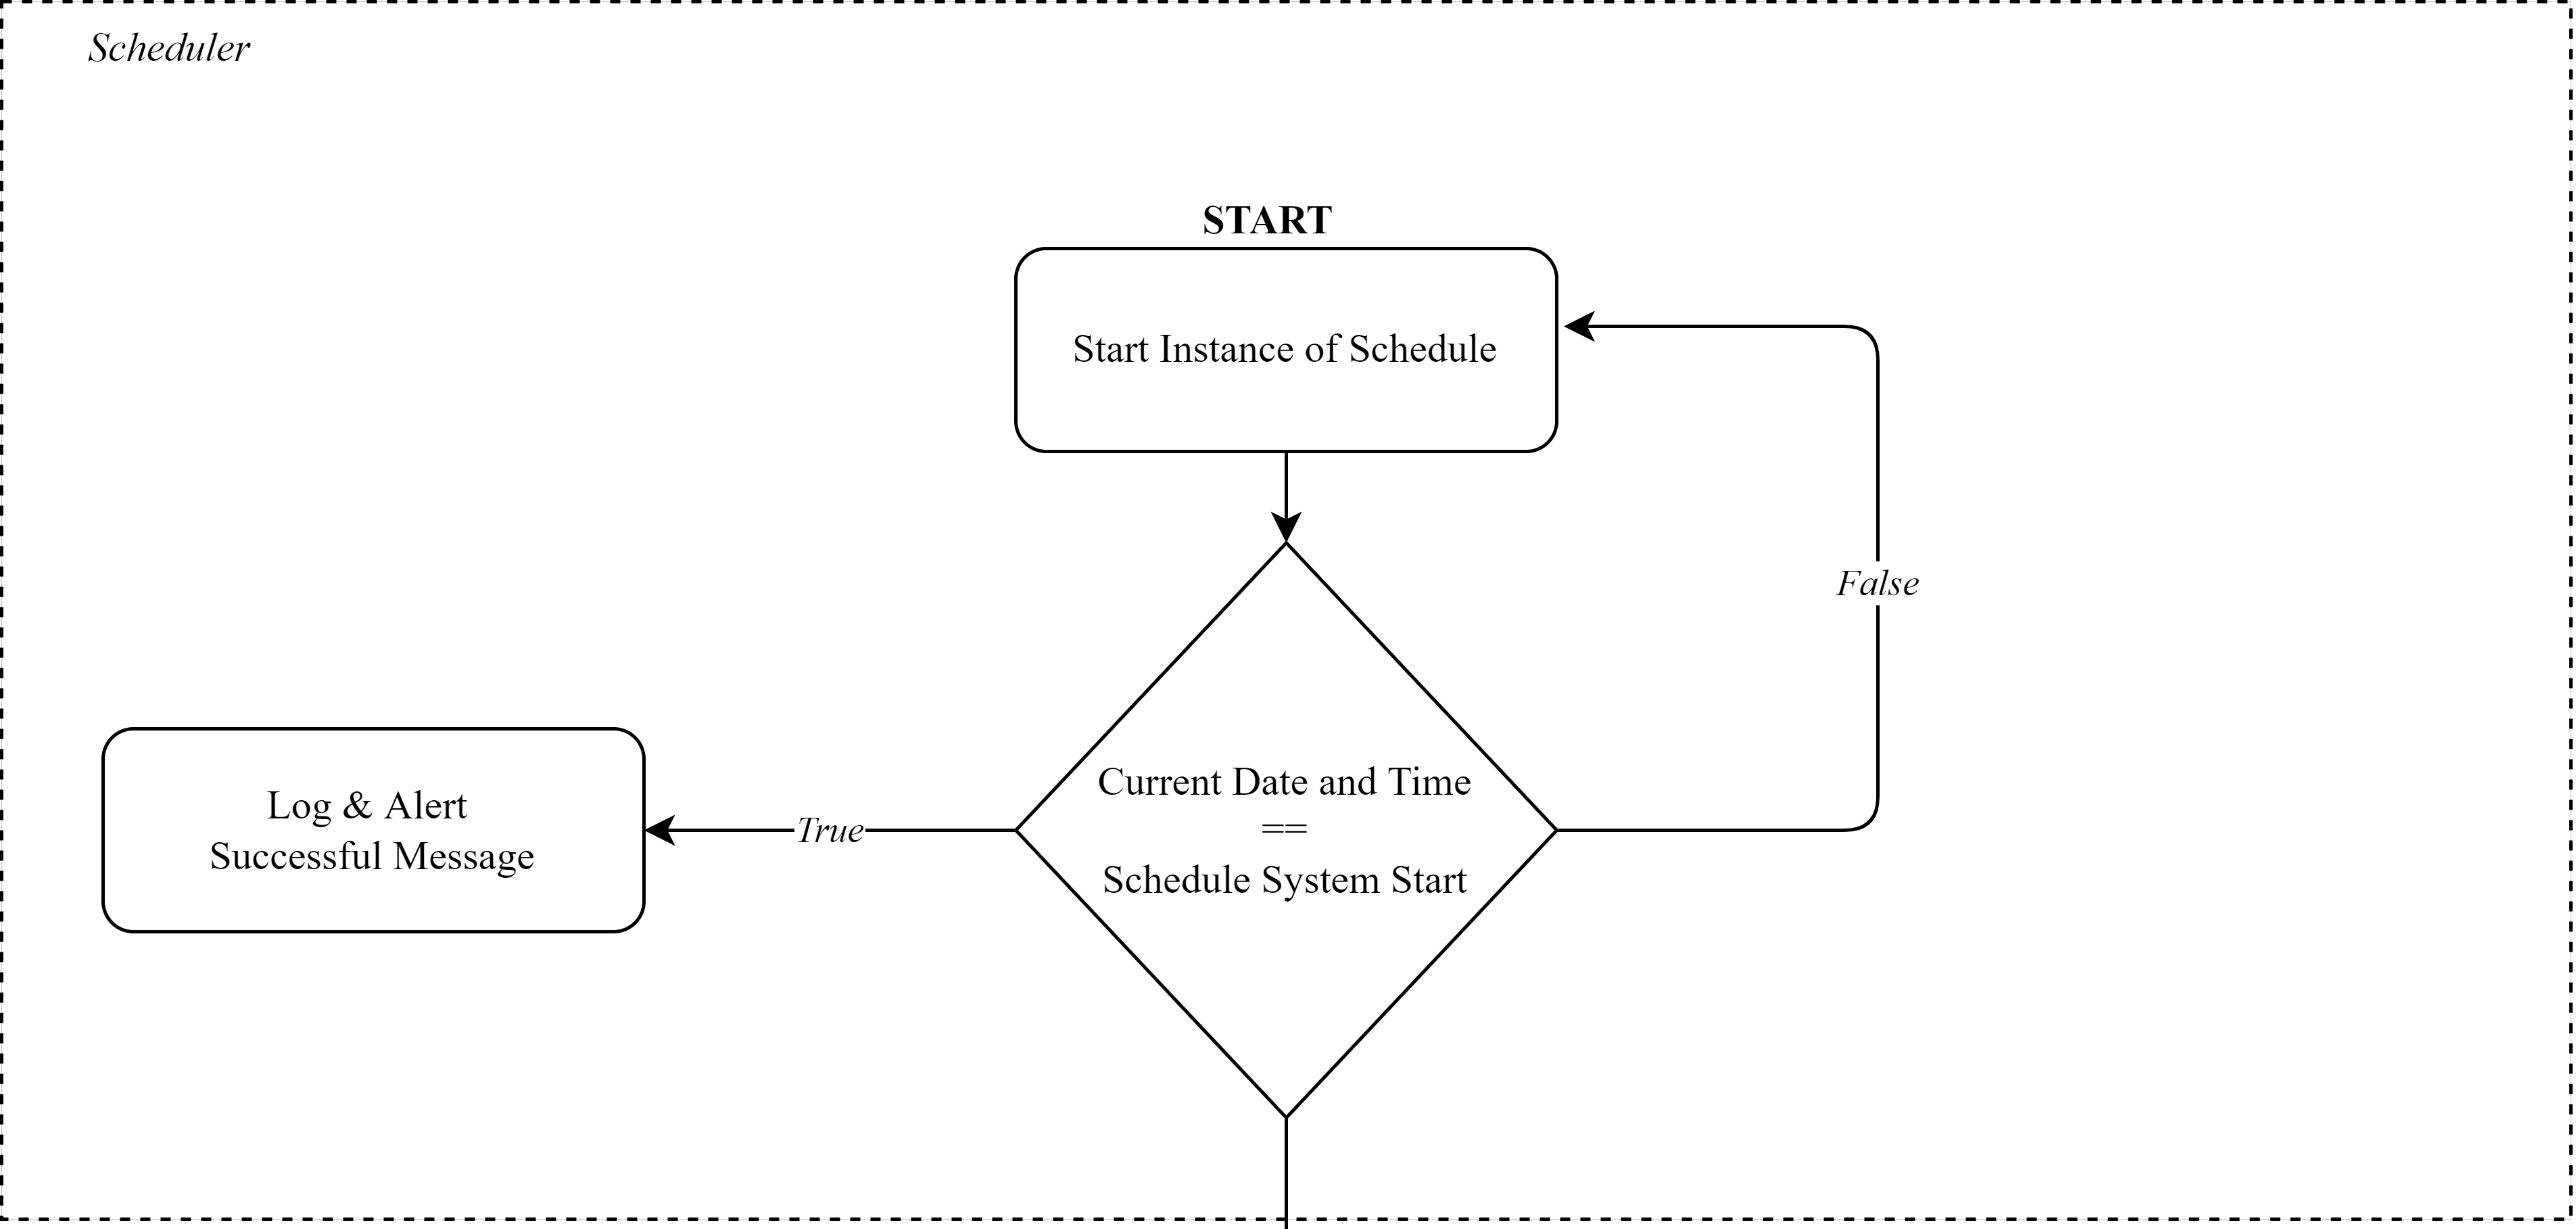
\includegraphics[width=1\textwidth]{./assets/Chapter_3/PFC/ProcessFlowchart_Scheduler.png}
    \caption{Overview of the Process Flow Diagram for the Scheduler}
    \label{fig:process_flowchart_scheduler}
\end{figure}
\FloatBarrier

% Data Collector
\subsubsection{Data Collector}
\label{subsubsec:data_collector}
The collection of end-of-day (eod) market data is the first process in the scheduled task.
\hfill \\
To collect eod market data, the system first looks for the EODHD API key, 
which is stored in system variables or provided by the user in the tools directory. 
If the system is unable to locate an API key, it logs the error and notifies the user before 
exiting the program.
\hfill \\
Once the API key is obtained, the system connects to the EOD market data provider and 
attempts to collect all market data five times. If it fails to collect data 
for the fifth time due to errors (i.e. incomplete payments, unstable network, and no established internet connection), 
the system logs the error, sends an alert to the user, and exits the program.
\hfill \\
All successful processes are also logged and sent to the command line interface to notify the user. 
Figure \ref{fig:process_flowchart_data_collector} depicts this, as well as the entire data collection process.
\hfill \\
The flow of processes discussed above can be observed in Figure \ref{fig:process_flowchart_data_collector}.
% Process Flowchart (Data Collector)
\begin{figure}[ht]
    \centering
    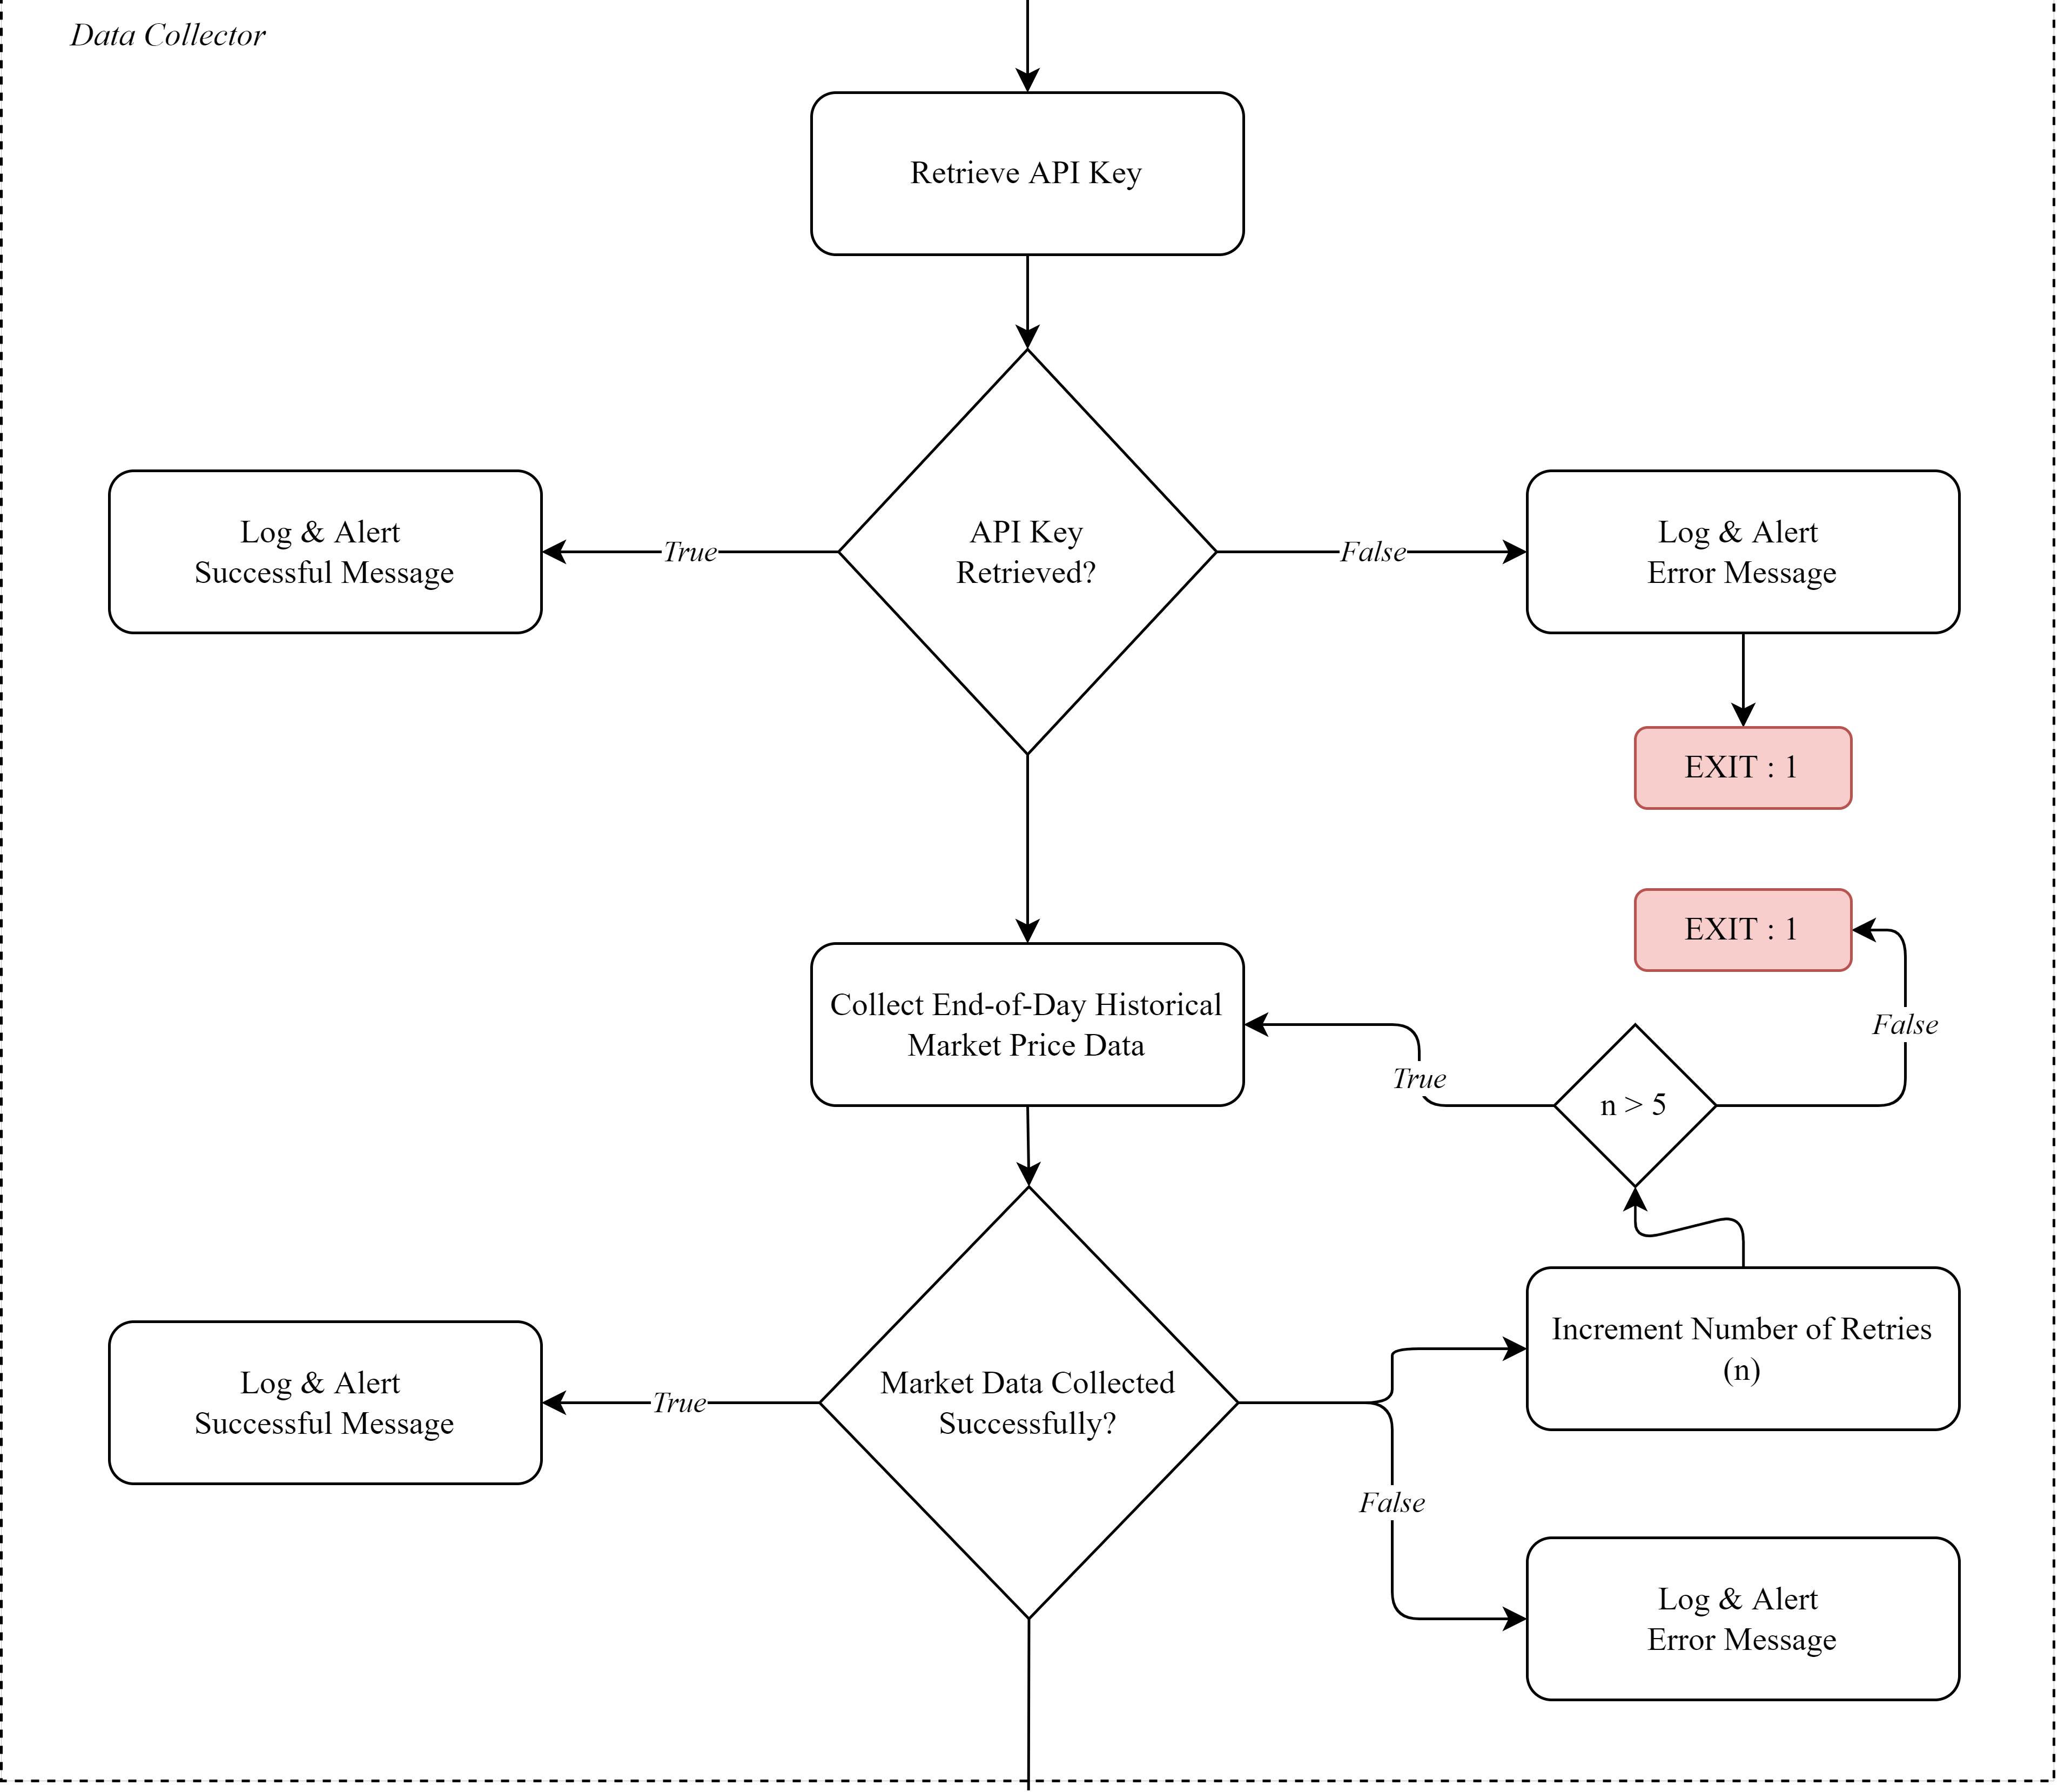
\includegraphics[width=1\textwidth]{./assets/Chapter_3/PFC/ProcessFlowchart_DataCollector.png}
    \caption{Overview of the Process Flow Diagram for the Data Collector}
    \label{fig:process_flowchart_data_collector}
\end{figure}
\FloatBarrier

% Data Processor
\subsubsection{Data Processor}
\label{subsubsec:ml_application}
Data Processor is a process that is divided into three subprocesses, as shown in 
Figure \ref{fig:process_flowchart_data_processor}.
% Process Flowchart (Data Processor)
\begin{figure}[ht]
    \centering
    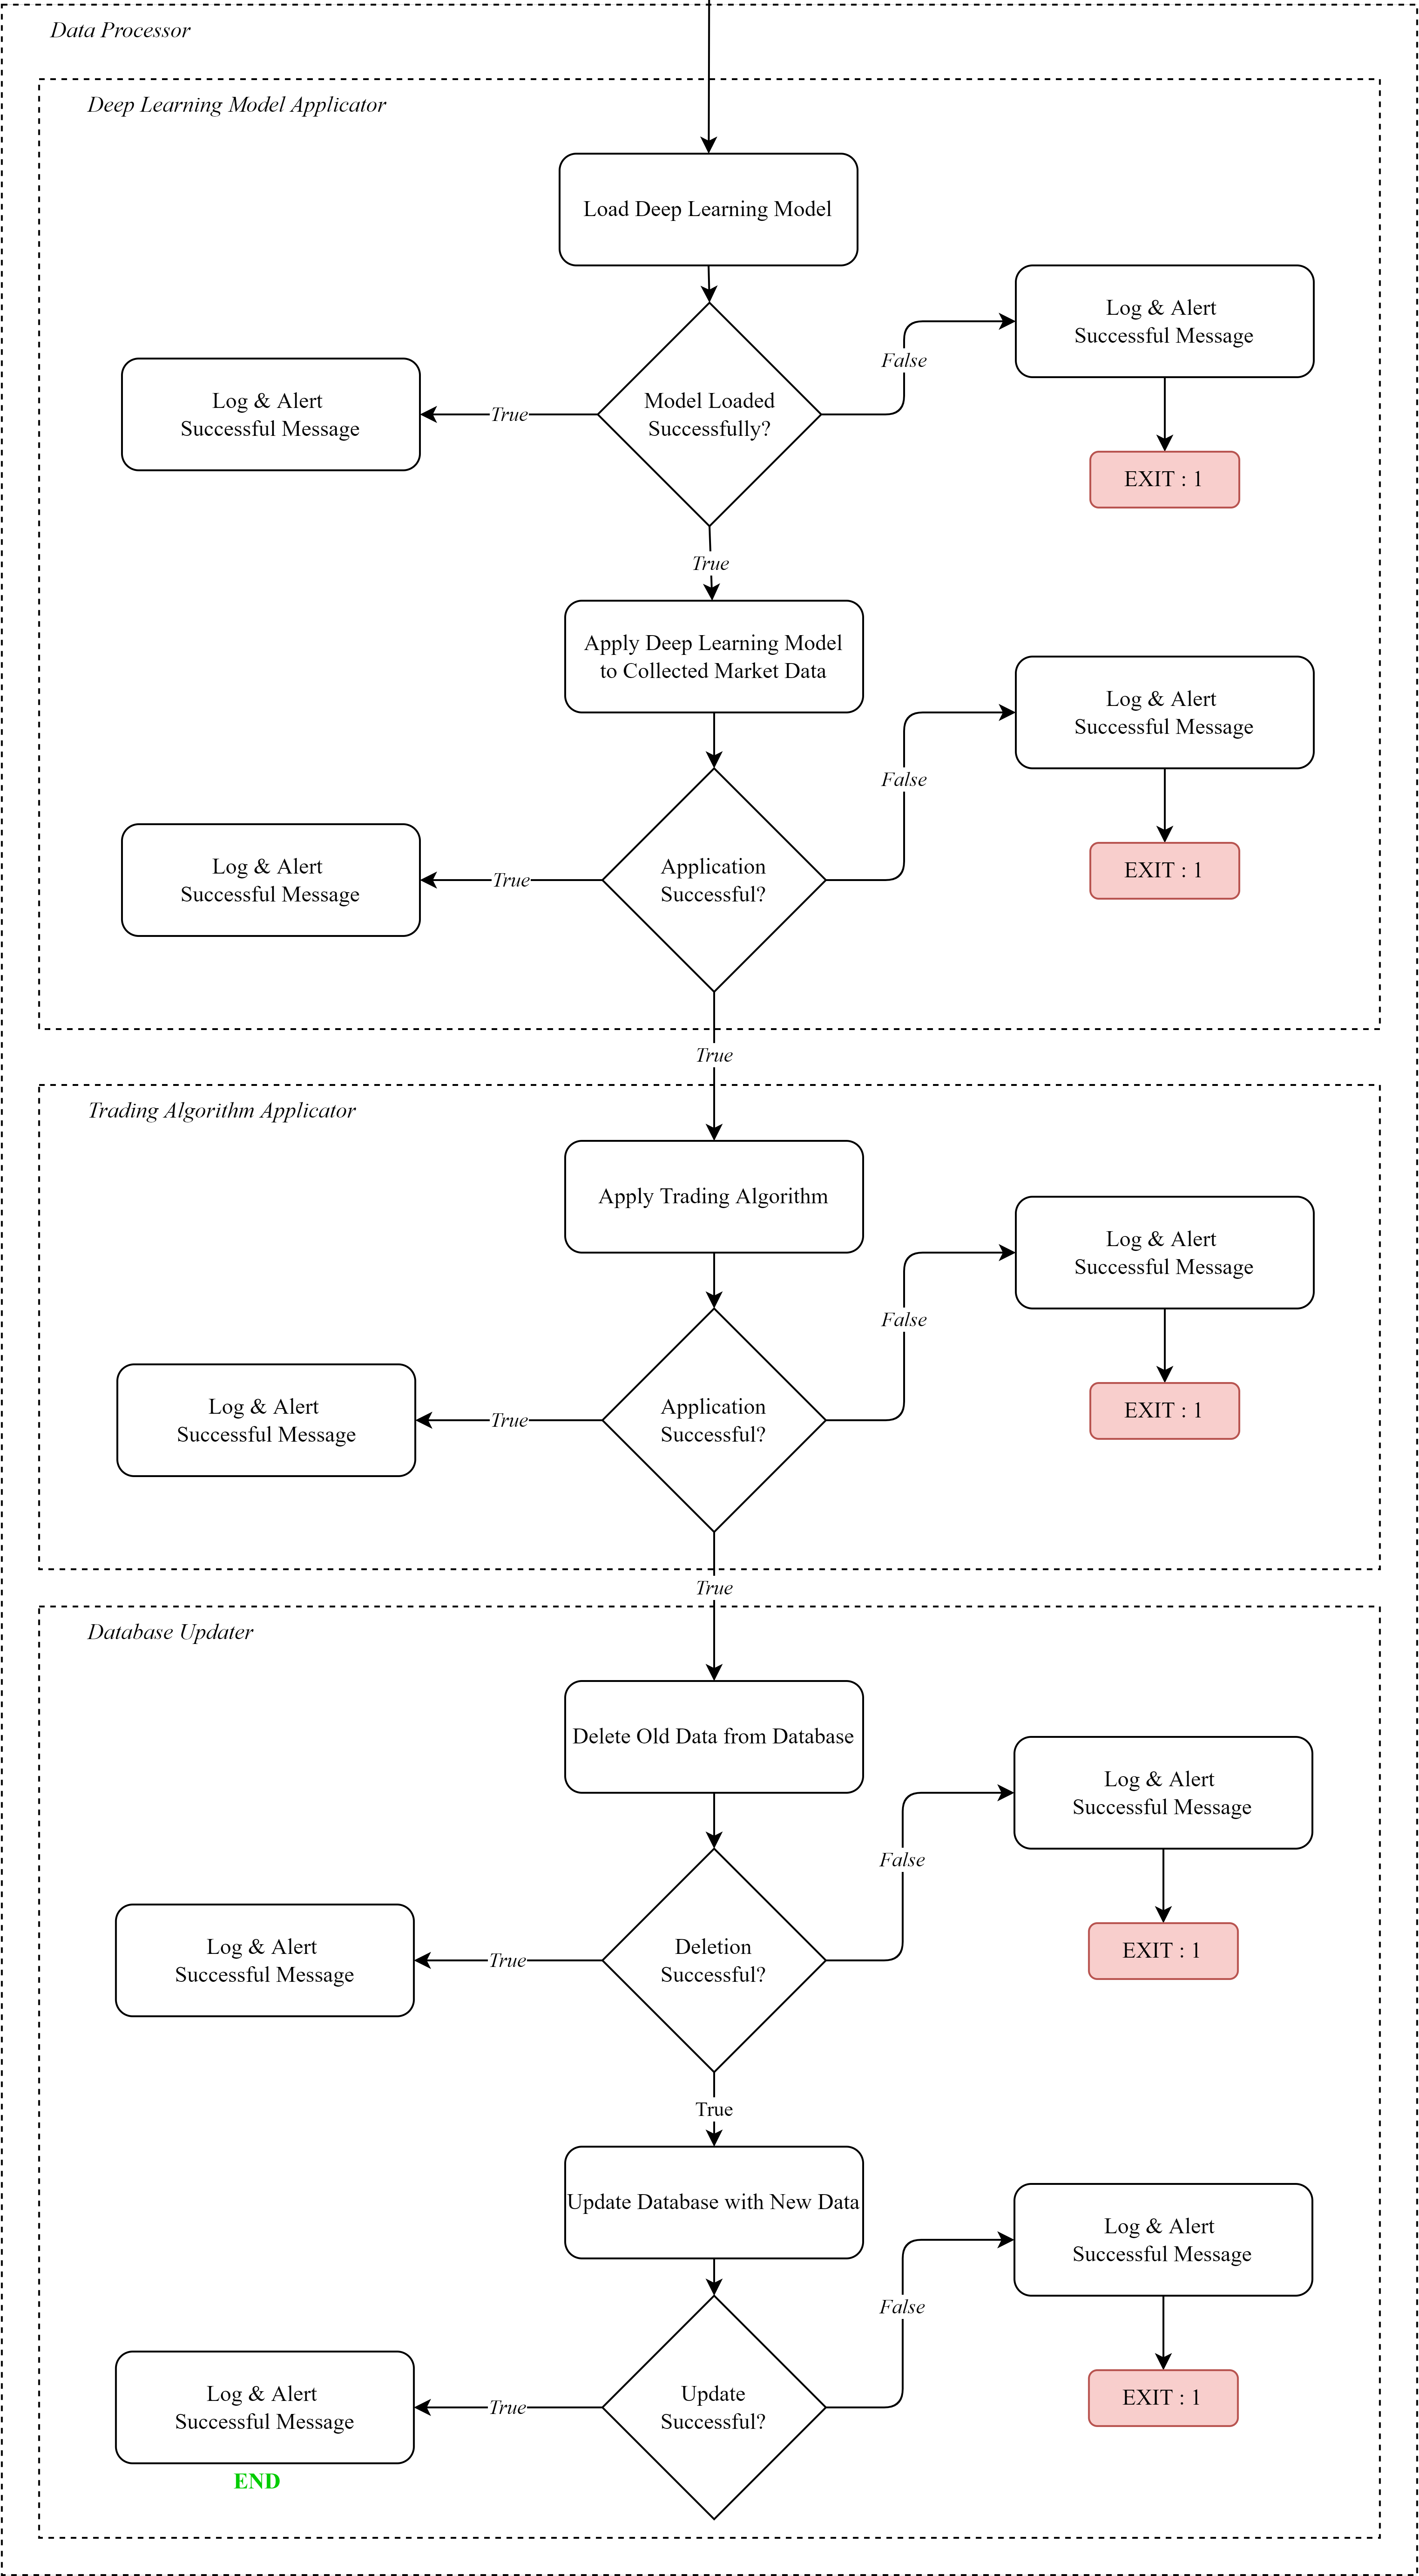
\includegraphics[height=0.8\textheight]{./assets/Chapter_3/PFC/ProcessFlowchart_DataProcessor.png}
    \caption{Overview of the Process Flow Diagram for Data Processor}
    \label{fig:process_flowchart_data_processor}
\end{figure}
\FloatBarrier

Where the three subprocesses are as follows:
\begin{itemize}
    \item[(a)] Deep Learning Model Applicator - This subprocess applies the deep learning model
    to the collected eod market data for each stock. Specifically, alamSYS applies the DMD-LSTM
    model developed as part of this special problem. This is done as illustrated in Figure
    \ref{fig:process_flowchart_dp_model_applicator}.
    % Process Flowchart (Data Processor - Deep Learning Model Applicator)
    \begin{figure}[ht]
        \centering
        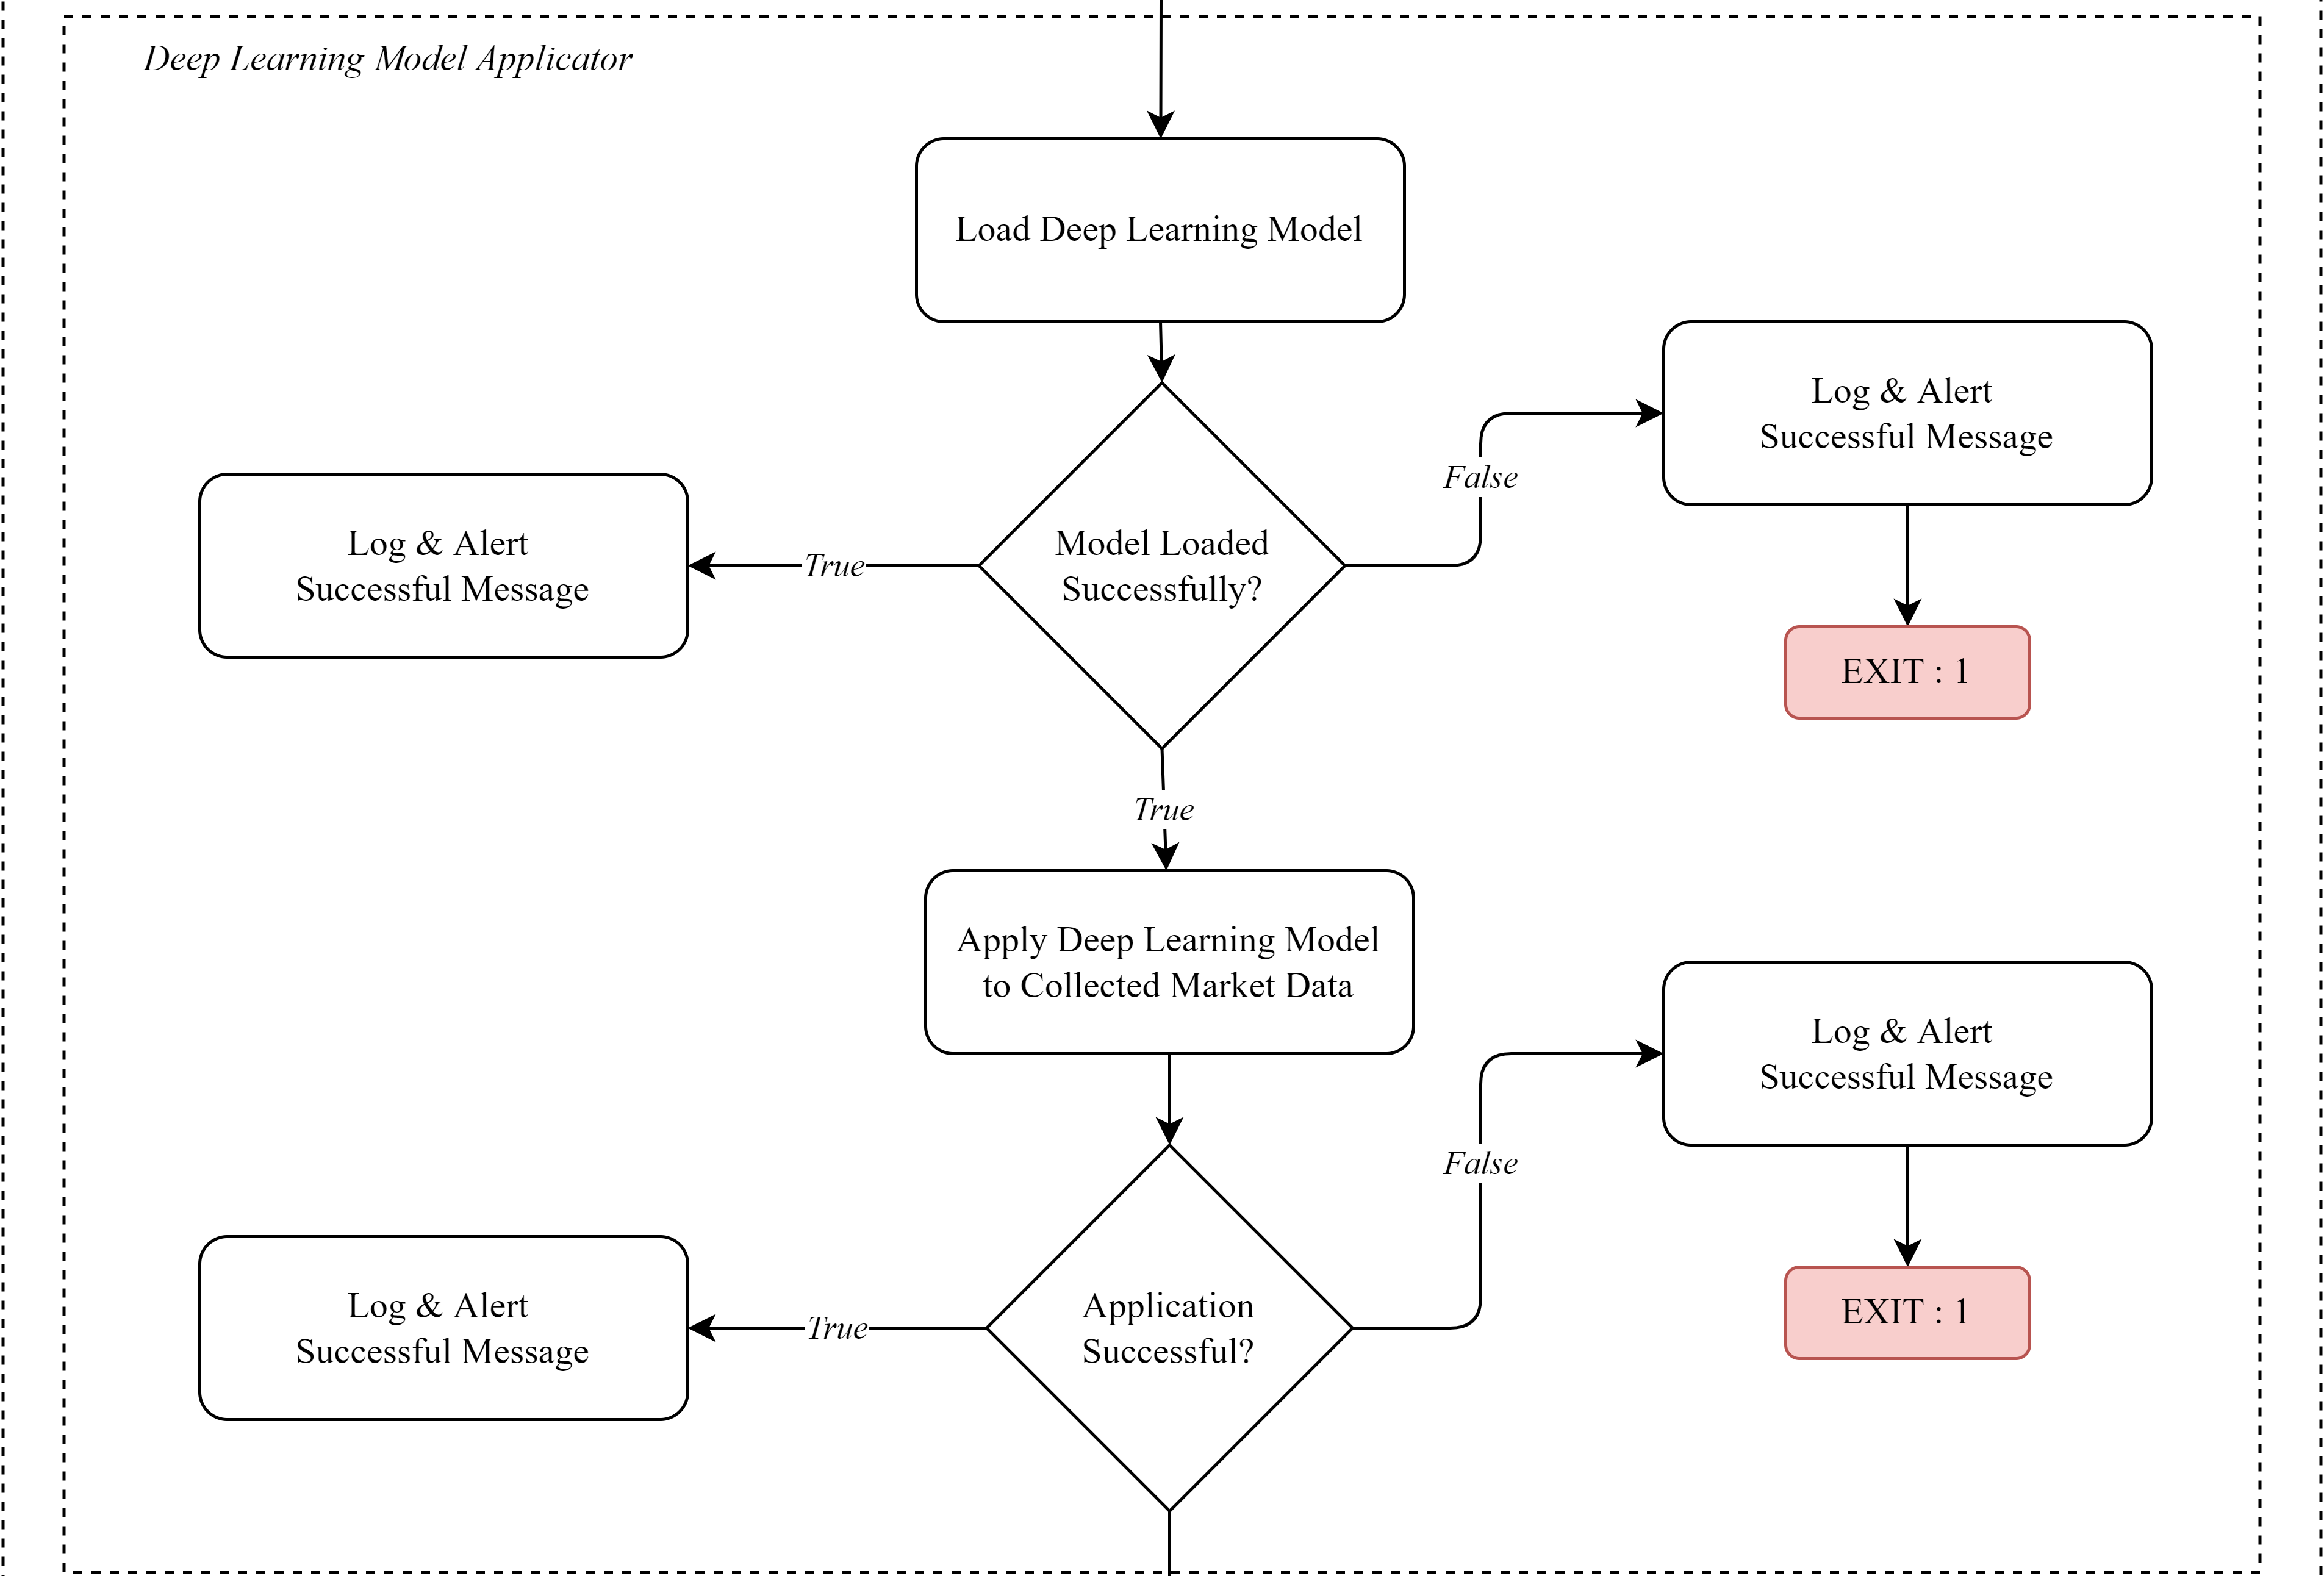
\includegraphics[width=1\textwidth]{./assets/Chapter_3/PFC/ProcessFlowchart_DataProcessor1.png}
        \caption{Overview of the Process Flow Diagram for the Deep Learning Model Applicator}
        \label{fig:process_flowchart_dp_model_applicator}
    \end{figure}
    \FloatBarrier
    \item[(b)] Trading Algorithm Applicator - This subprocess applies the trading algorithm
    to the output data from the deep learning model applicator. Specifically, alamSYS applies
    ALMACD algorithm developed as part of this special problem. This is done as illustrated in Figure
    \ref{fig:process_flowchart_dp_trad_algo_applicator}.
    % Process Flowchart (Data Processor - Trading Algorithm Applicator)
    \begin{figure}[ht]
        \centering
        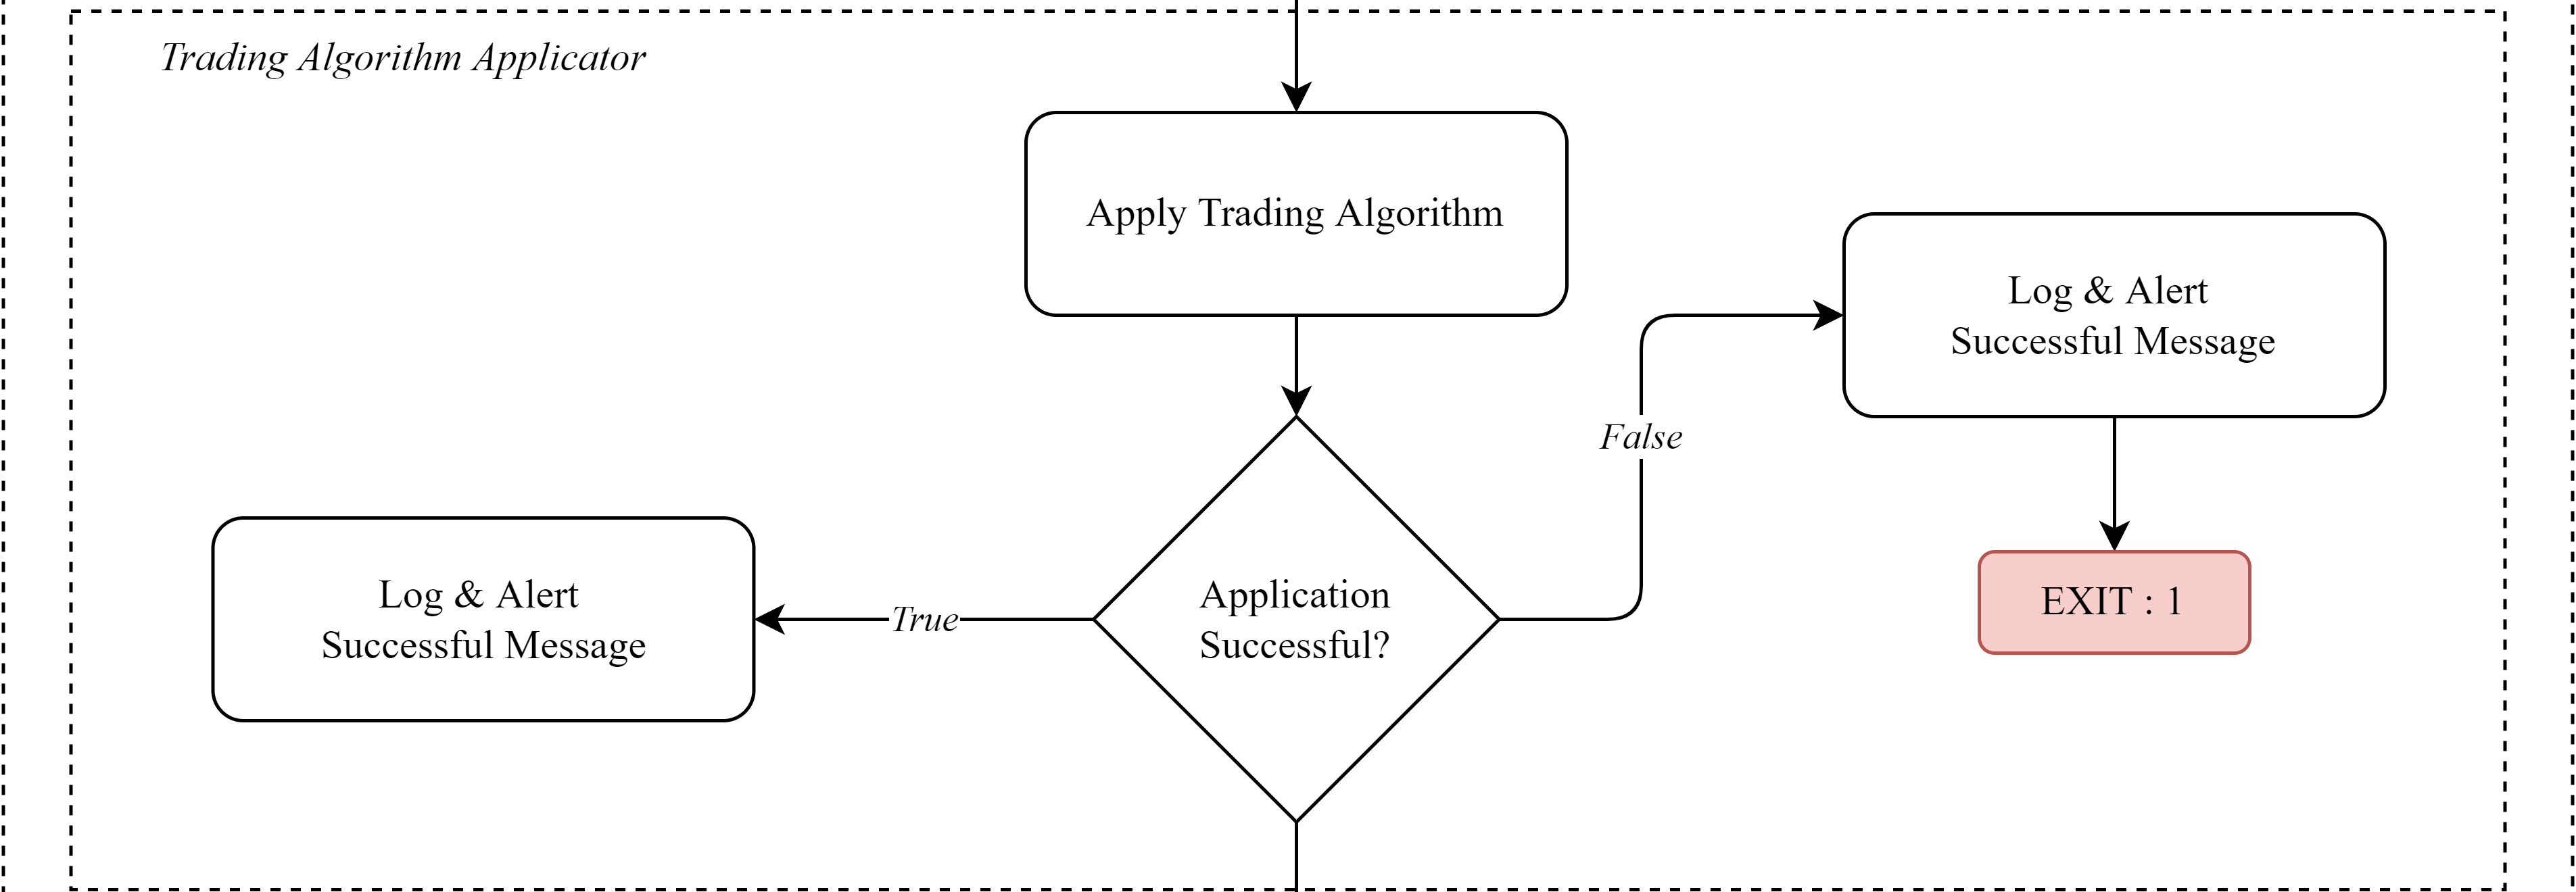
\includegraphics[width=1\textwidth]{./assets/Chapter_3/PFC/ProcessFlowchart_DataProcessor2.png}
        \caption{Overview of the Process Flow Diagram for the Trading Algorithm Applicator}
        \label{fig:process_flowchart_dp_trad_algo_applicator}
    \end{figure}
    \FloatBarrier
    \item[(c)] Database Updater - This subprocess updates the database with the output data from
    the trading algorithm applicator. This is done as illustrated in Figure \ref{fig:process_flowchart_db_updater}.
    % Process Flowchart (Data Processor-Database Updater)
    \begin{figure}[ht]
        \centering
        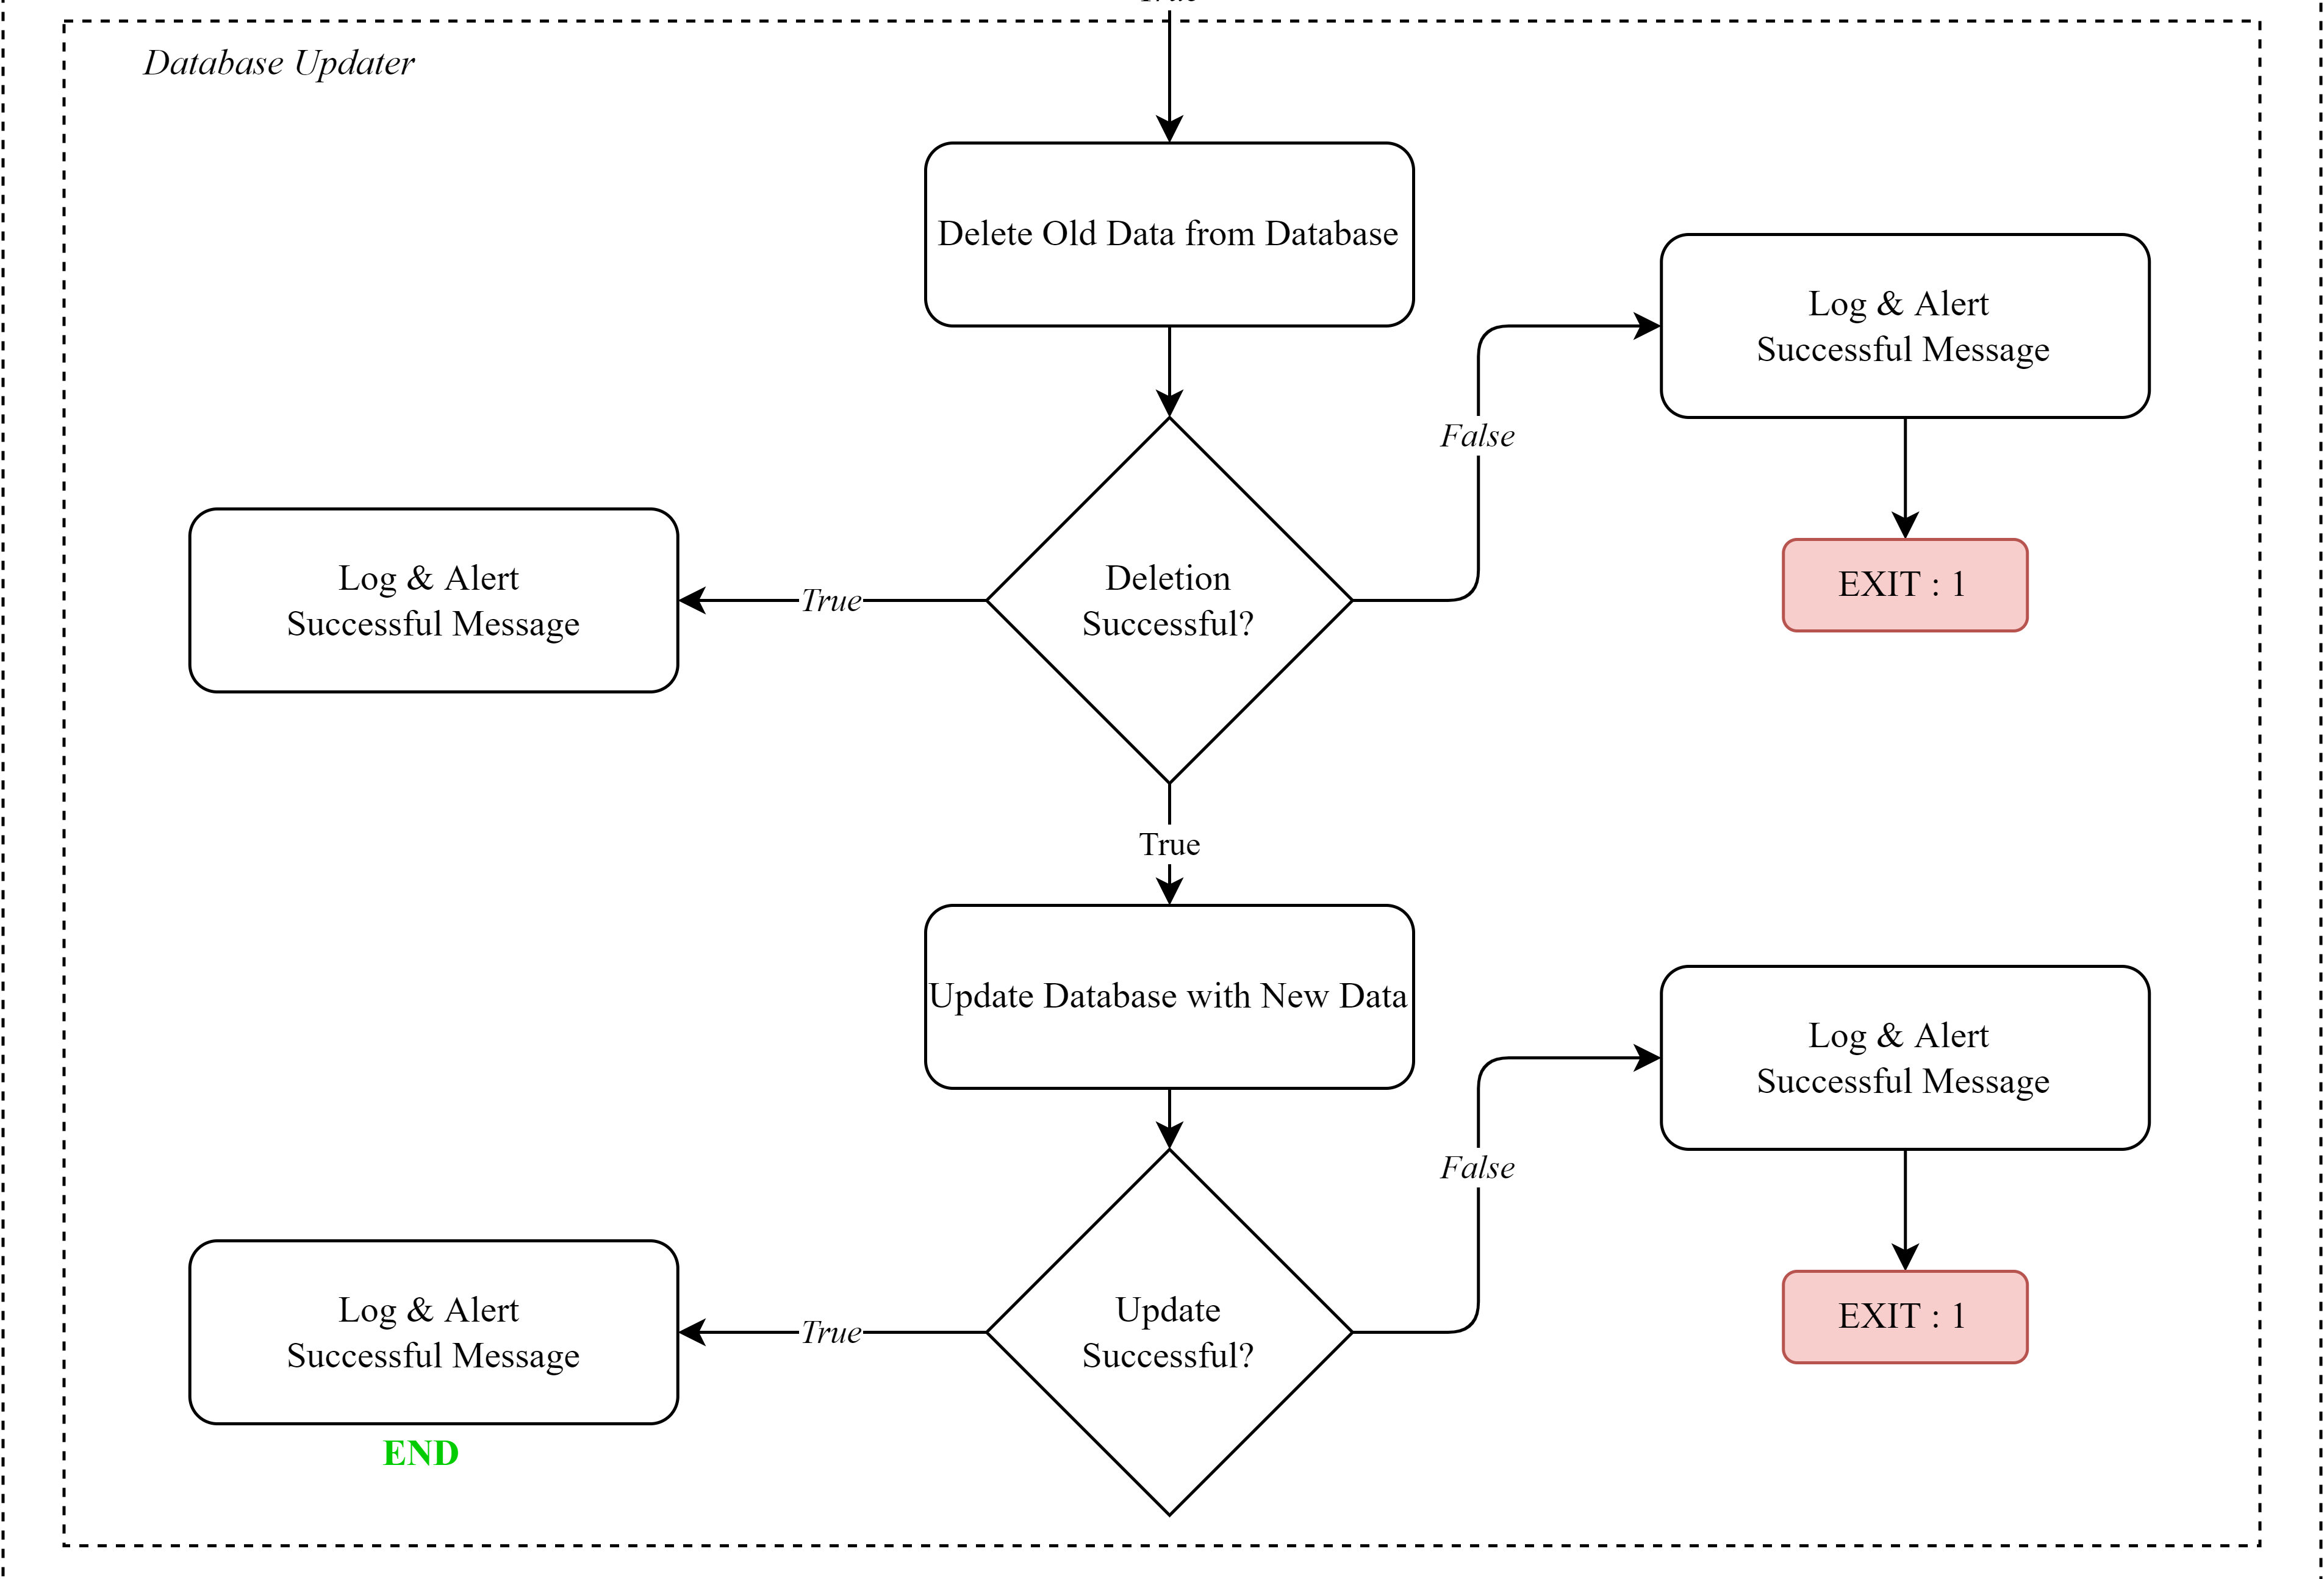
\includegraphics[width=1\textwidth]{./assets/Chapter_3/PFC/ProcessFlowchart_DataProcessor3.png}
        \caption{Overview of the Process Flow Diagram for the Database Updater}
        \label{fig:process_flowchart_db_updater}
    \end{figure}
    \FloatBarrier
\end{itemize}
